\subsection{Architecture de LiveScaler}

\begin{figure}[htbp]
  \centering
	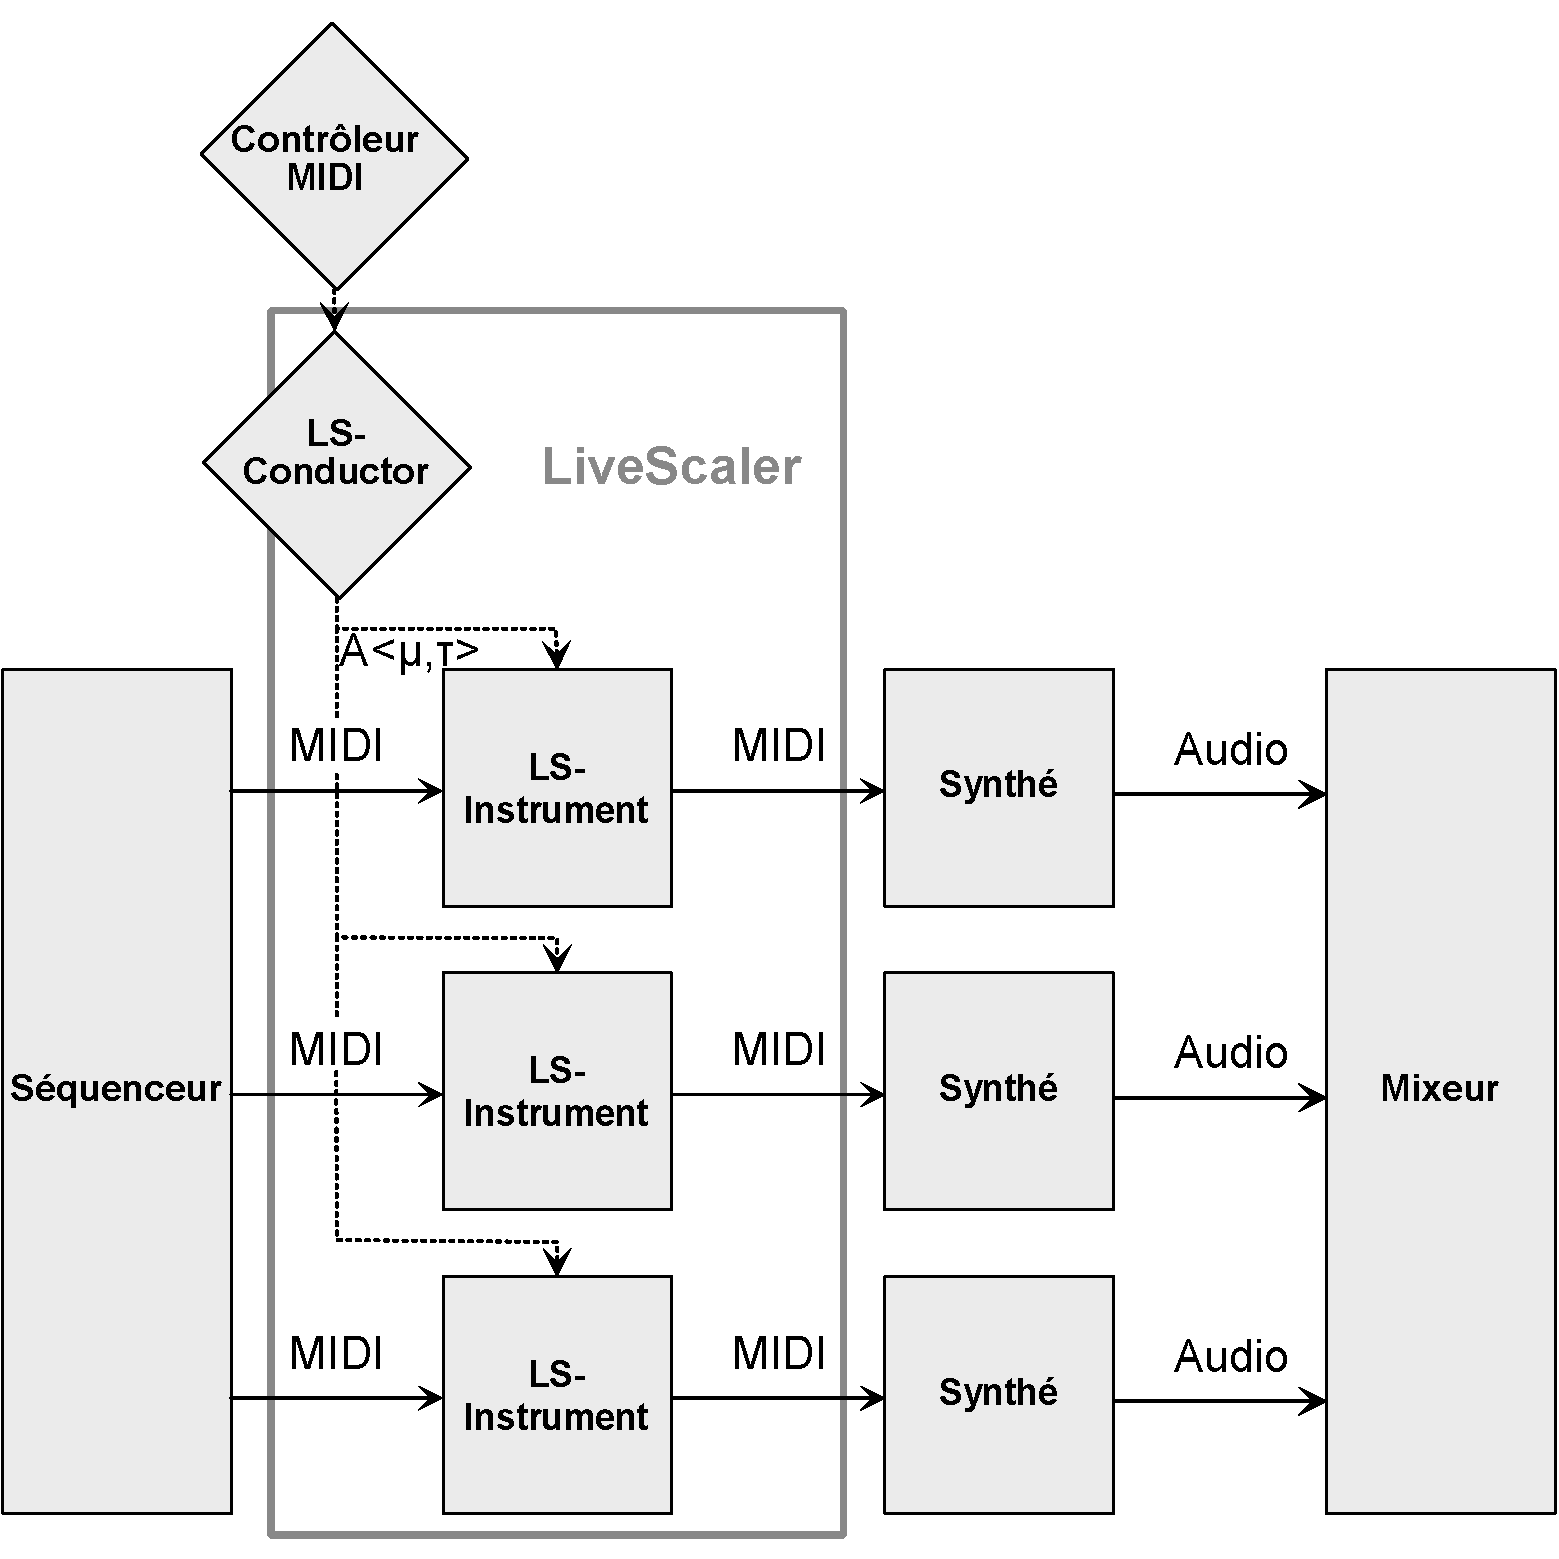
\includegraphics[width=\columnwidth]{architecture-LS.pdf}
  \caption{Architecture de Live Scaler\label{fig:archi}}
\end{figure}

LiveScaler fonctionne à la manière d'un orchestre dont le  DJ serait le chef. Chaque piste MIDI contenant un instrument virtuel (synthétiseur, sampleur, etc.) est un instrumentiste de l'orchestre. On souhaite que sur un geste du DJ, chaque instrument virtuel interprète différemment sa partition, c'est à dire le flux MIDI qu'il reçoît. Dans le cadre de LiveScaler, le DJ envoie les paramètres d'une transformation affine à tous les instruments simultanément et ceux-ci doivent appliquer cette transformation dès qu'ils la reçoivent.

L'implémentation de LiveScaler est donc séparée en deux outils interdépendants : 
\begin{enumerate}
  \item une interface (appelée \emph{Conductor}, en référence à l'analogie avec l'orchestre) qui récupère les entrées de l'utilisateur (ici le DJ) et les convertit en paramètres d'une transformation affine puis envoie ces paramètres à toutes les instances de \emph{Instrument}.
  \item un plug-in MIDI appelé \emph{Instrument} qui transforme le flux MIDI entrant en appliquant à toutes les notes la transformation affine dont les paramètres ont été reçus de \emph{Conductor}.
\end{enumerate}
La Figure \ref{fig:archi} illustre l'architecture globale de LiveScaler.

On distingue également les paramètres \emph{locaux}, qui sont propres à chaque instrument, et les paramètres \emph{globaux}, qui sont reçus du chef d'orchestre et donc communs à tous les instruments. Dans le cadre des transformations affines, les paramètres $\mu$, $\tau$, $\alpha$  et $\beta$ sont globaux, il correspondent dans une certaine mesure à l'harmonie actuelle du morceau. Quant à $\delta^-$ et $\delta^+$, ils sont locaux et peuvent être adaptés à la tessiture de l'instrument.
\begin{figure*}[h]
  \centering
  \begin{subfigure}{0.83\textwidth}
    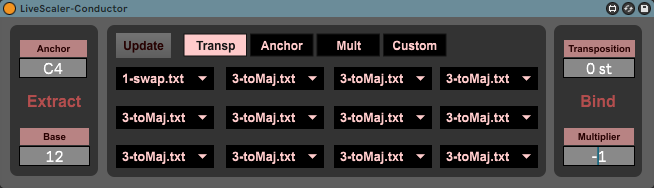
\includegraphics{Figures/LS-Conductor-UI.png}
  \end{subfigure}
  \begin{subfigure}{0.15\textwidth}
    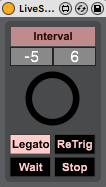
\includegraphics{Figures/LS-Instrument-UI.png}
  \end{subfigure}
  
  \caption{Interface graphique de LiveScaler (\emph{Conductor} à gauche  et  \emph{Instrument} à droite) }
  \label{fig:LiveScalerUI}
\end{figure*}
